%% This is an example first chapter.  You should put chapter/appendix that you
%% write into a separate file, and add a line \include{yourfilename} to
%% main.tex, where `yourfilename.tex' is the name of the chapter/appendix file.
%% You can process specific files by typing their names in at the 
%% \files=
%% prompt when you run the file main.tex through LaTeX.
\chapter{Background}

This chapter provides a brief survey of existing approaches to reinforcement learning.
It starts by describing Markov Decision Processes, the class of stochastic
optimization problems used to model reinforcement learning.
It then discusses existing work on solving Markov Decision Processes, placing
an emphasis on the ideas most relevant to this thesis.

\section{Markov Decision Processes}
A Markov Decision Process (MDP) is an optimization problem formulation 
often described in terms of an agent acting on its environment \cite{put}.
The agent's actions cause stochastic changes in the state of the environment
and the agent gets rewarded for effecting desirable changes.

Single player video games with an element of chance are naturally modelled
as MDPs.
The agent is the player and the environment is the game world.
The actions are the things the player can do within the rules of the game, and
the reward is the player's score.

MDPs were originally studied in the context of industrial applications.
Over the past few decades, however, they have been adopted by the AI
community to model larger and more complicated optimal control problems.

Formally, an MDP can be expressed as a tuple $<S,A,T,R,\gamma>$ where
\begin{itemize}
  \item$S$ is a (possibly infinite) set of possible states for the environment.
  \item $A$ is a finite set of actions the agent can take.
  \item $T:S \times A \times S \to [0,1]$ is a function expressing the
    probability that some action will result in a particular state transition.
  \item $R:S \times A \times S \to \mathbb{R}$ is a function expressing the
    reward the agent gets for each state transition it can cause.
  \item $\gamma \in [0,1)$ is a discount factor specifying how much the
    agent prefers immediate rewards to rewards that occur in the future.
\end{itemize}

The mechanics of an MDP are as follows. The agent starts the process in some
start state, $s_0$.
At every subsequent time step, $t$, the agent is allowed to choose an action,
$a_t$.
This causes the state to change to state $s_{t+1}$ with probability
$T(s_t,a_t,s_{t+1})$.
The agent receives a reward $r_t = R(s_t,a_t,s_{t+1})$ for the
transition.
Note that the reward and transition functions, $R$ and $T$, are independent
of the time step $t$.
They are also independent of the state and action history of the process.
This is known as the Markov property and it makes the optimal action
depend only on the current state of the world.

The rule the agent uses for deciding which action to take for a given state
is called its policy, $\pi$.
The lifetime reward the agent expects to get when using $\pi$ starting from
state $s$ is denoted
$V^\pi(s) = E\big[\sum_i \gamma^i r_i | s_0 = s, a_i = \pi(s_i)\big]$.
The objective of the agent is to maximize its lifetime expected reward.
This means finding a policy, $\pi^*$, such that
$V^{\pi^*}(s) = \max_\pi V^\pi(s)$ for all states $s$.

In reinforcement learning, the reward and transition functions are assumed to
be unknown. The agent must learn optimal behaviour by observing sample
rewards and transitions.
For more details see Sutton and Barto \cite{rlai}.
In this thesis, I assume that the agent is given a batch of sample
transitions from which to deduce optimal behaviour.

\subsection{Solving MDPs}
A popular approach to solving MDPs is to approximate the value function
by starting from some initial estimate and iteratively updating it to be
consistent with the rewards attainable in a single step.
This technique is known as value iteration.
Other common techniques are policy iteration and linear programming.
Since this thesis deals with improving value iteration techniques,
that is the only approach discussed below.

As described in the previous subsection, each state, $s$, in an MDP has a
value, $V^{\pi^*}(s)$, which is the expected return when starting in $s$ and
acting optimally.
It is also convenient to think in terms of the value of a state action pair,
$Q^{\pi^*}(s,a)$, which is defined as the expected return when taking action,
$a$, in state, $s$, then acting optimally forever after.
This function is referred to as the Q-Value.
It should be apparent that the value function is the upper envelope of the
Q-Values, $V^\pi(s) = \max_a Q^\pi(s,a)$.
We know, thanks to Bellman, that acting greedily with respect to Q-Values is
optimal \cite{put}.

If the set of states is finite, the value function can be computed by a
dynamic program that iteratively enforces the relation
$$ Q(s,a) = \sum_{s'} T(s,a,s')\big[R(s,a,s') + \gamma V(s')\big] $$
in what is known as a Bellman update.

Solving MDPs with continuous state spaces\footnote{The number of actions is
still assumed to be finite.} is less straightforward.
In the general case, the solution to a continuous MDP is uncomputable.
This thesis is focused on a restricted class of continuous MDPs that describe
a continuous time control problem where the state is sampled at some regular
time interval, $\Delta t$.
Such MDPs of are often solvable by
approximate value iteration because they tend to have smooth transition and
reward functions.
For convenience, the state space is assumed to lie within the unit cell
$[0,1]^d$.
As we will see in the results section, this formulation is general enough to
represent many problems of interest to the RL community.

Value iteration algorithms for such MDPs can broadly be classified as
parametric or non-parametric.
Parametric approaches assume the Q-Values have some functional form.
Notable instances are LSTD \cite{lstd} and SARSA \cite{sarsa}, which fit the
Q-Values with a linear combination of basis functions, and fitted Q-iteration
\cite{fqi} which fits the Q-Values with a neural network.
If the assumed form is appropriate, parametric value iteration
can produce optimal policies from very little data.
On the other hand, no amount of data
can help parametric value iteration produce a good policy when the assumed
form is not appropriate.
Parametric approaches have had considerable success in practice \cite{rlai}
\cite{rlsa}
but lack some desirable convergence guarantees \cite{five} \cite{three}.

Alternatively, non-parametric methods create a value function representation
directly from the data.
This allows the complexity of the fit to scale naturally with the sample size.
Non-parametric approaches have the added benefit of being more robust to
some aspects of dimensionality.
If the data lies on a low dimensional manifold in a high dimensional space,
the amount of data needed for a non-parametric approach is proportional to
volume of the manifold; however, without a basis constructed specifically for
the manifold, a parametric approach would need a number of bases exponential
in the dimensionality of the embedding space.

Though the techniques presented in this thesis could be applied in a parametric
setting, the focus is on non-parametric techniques; therefore, only
non-parametric approaches are discussed in the remainder of this thesis.
Applications to parametric settings are left for future work.
What follows is a survey of prevailing non-parametric approaches.

\section{Kernel Based Reinforcement Learning}
KBRL \cite{kbrl} is a non-parametric value iteration algorithm for
continuous MDPs.
It is a three-step process that solves the MDP using a set of sample
transitions.
The first step constructs a finite approximation of the MDP from the samples.
The second step solves the finite MDP.
Finally, the third step interpolates the solution to the entire state space.

KBRL provides numerous desirable theoretical guarantees.
It is statistically consistent---using more data improves performance.
It also converges to a unique solution.
The main drawback of KBRL is that it can be computationally intensive.

\subsection{Overview}
KBRL takes as input a set of sample transitions, 
$S^a = \{ (s^a_k, r^a_k, \hat s^a_k) | k = 1, \ldots, n_a \}$, resulting from
each action, $a$. 
From these transitions, KBRL constructs a finite MDP $M'=<S',A,T',R',\gamma>$. 
The new state space, $S'$, is the set of sample transitions. 
$|S'| = n = \sum_a n_a$. 
The new reward function\footnote{
The * character is used when the element at that position is irrelevant.
This is not standard notation in the literature and is used in this
thesis for clarity.} is $R'((*,*,*), *, (*,r^a_i,*)) = r^a_i$.
The new transition function $T'$ is defined as 
\[
 T'((*,*,\hat s^{a}_i), a', (s^{a''}_j,*, *)) = \left\{
  \begin{array}{lr}
    0 & \mathrm{if}\ a' \neq a'' \\
    \kappa_a(\hat s^a_i, s^{a''}_i) &  \mathrm{otherwise,}
  \end{array}
\right.
\]
where $\kappa_a(\cdot, \cdot)$ is some similarity function.
The constraints on $\kappa_a$ are discussed in the next subsection; for now
just assume that each $\kappa_a$ is a Gaussian with some unspecified
bandwidth, $\mathrm{exp}(\frac{-||s_1-s_2||^2}{b^2})$, normalized so that
$\sum_i \kappa_a(s,s^a_i) = 1$ for all $s$.

After constructing $M'$, KBRL solves it using value iteration to get $Q'$,
the Q-Values of $M'$.
KBRL generalizes these values to $M$ using the equation
$$Q(s,a) = \sum_{(s',r,\hat s) \in S^a}
\kappa(s,s')\big[r + \gamma V'((s',a,\hat s))\big].$$

\subsection{Details, Properties, and Assumptions}
KBRL uses local averaging to construct the finite model $M'$.
The functions $\kappa_a$ are kernel smoothers that set the weights
for the averaging.
For an intuition about how this works, consider the following example.

Assume the sample transitions are the ones shown in Figure 2-1.
There are 9 sample transitions over two actions, $a_1$ and $a_2$.
The letters $x$ and $y$ are used to denote the start and end, respectively,
of a transition.
Superscripts denote the action taken and subscripts index the transitions.
The model built by $M'$ assumes that taking $a_i$ from anywhere 
will result in a transition to some $y^i_j$. The transition probability is
$T'(s,a_i, y^i_j) \propto \mathrm{exp}(\frac{-||s-x^i_j||^2}{b^2})$.
For a sufficiently small bandwidth, $b$, the model will predict that
taking $a_1$ from the state, $s$, shown in the figure will lead to
$y^1_1$ with high probability. This is because $x^1_1$ is
closer to $s$ than any of the other sample points where action $a_1$
is taken.
For large bandwidth, the transition probability will approach uniform over
$\{y^1_j | j= 1,2,3,4\}$.
KBRL will never assign positive probability to $a_1$ causing a transition
into any $y^2_j$.

\begin{figure}[h!]
  \centering
    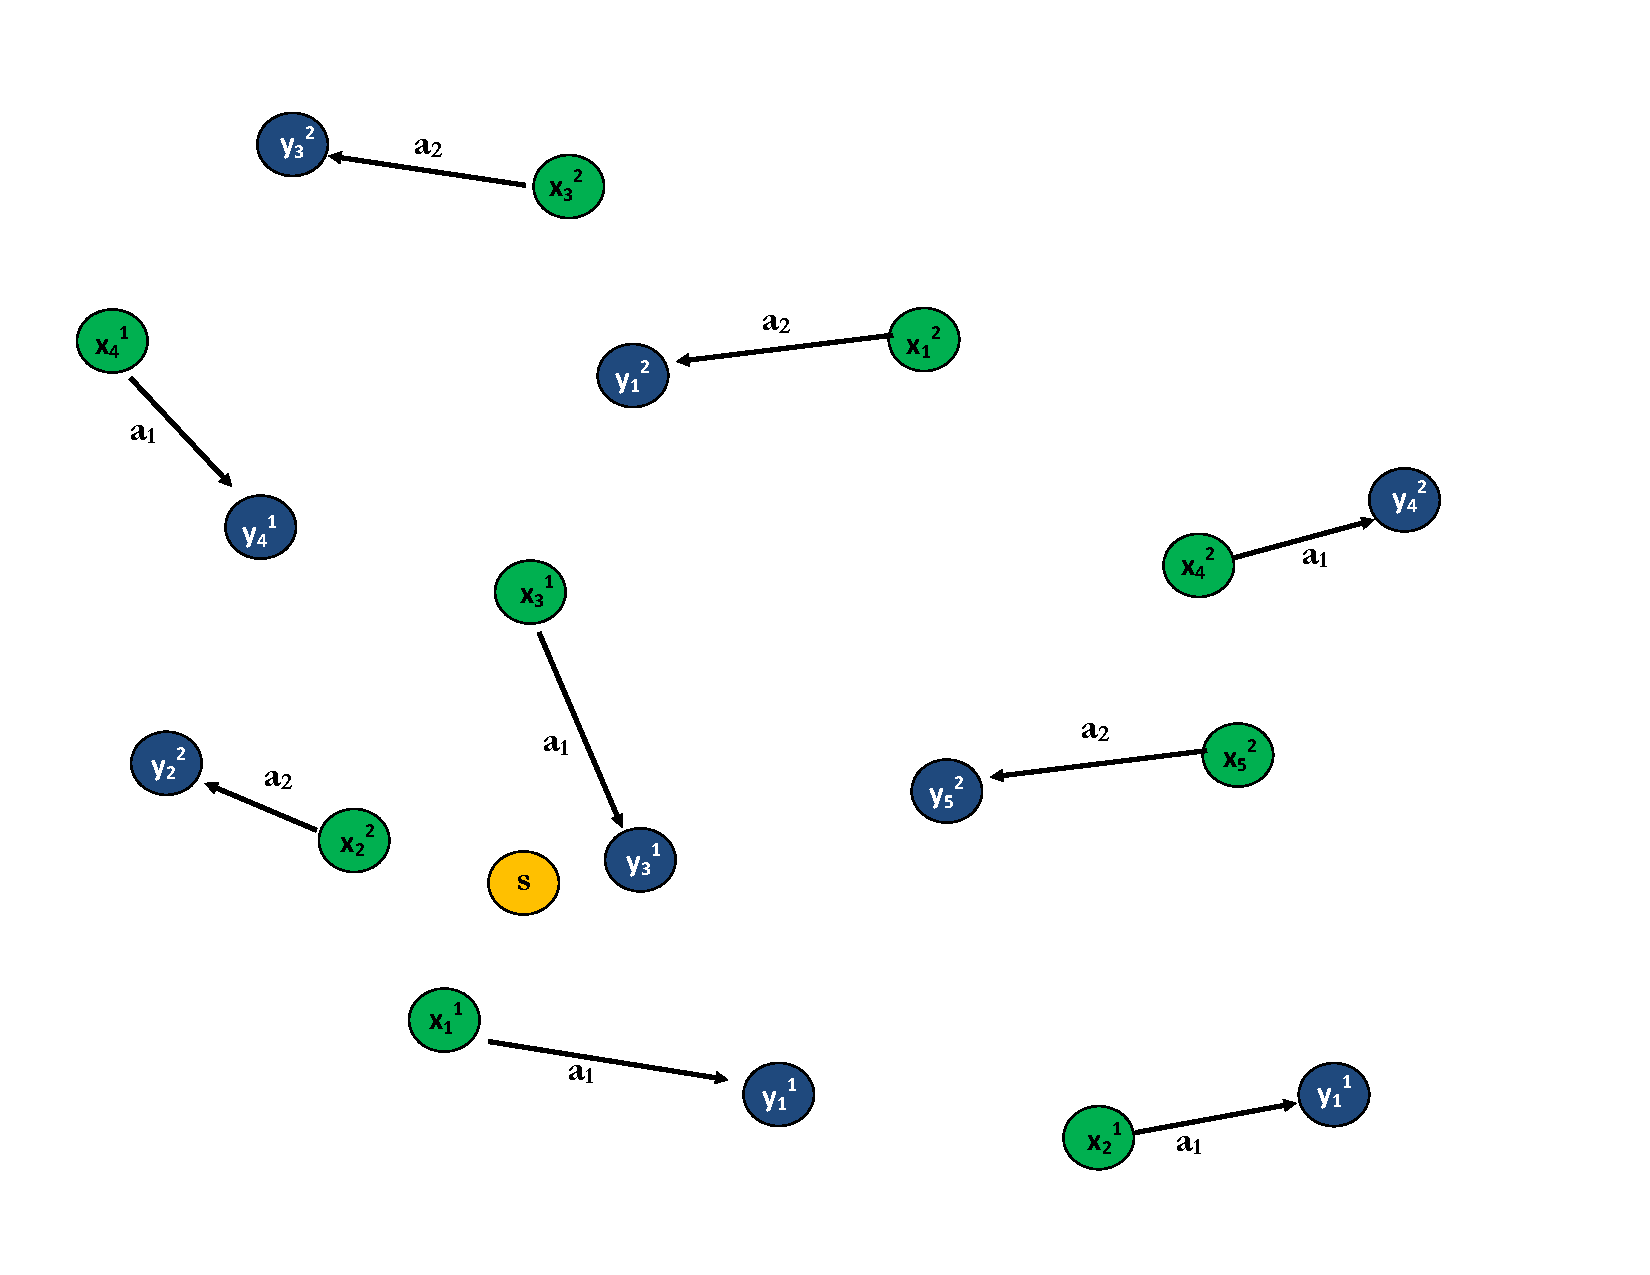
\includegraphics[width=120mm, height=108mm]{figs/kbrlexpl.pdf}
  \caption[Explanation of the the KBRL finite model]{An example set of transitions.
      Arrows are labelled with the action taken.
      For bandwidths near $0$, KBRL assumes $a_1$ takes $s$ to $y^1_1$ and
      that $a_2$ takes $s$ to $y^2_2$ with probability near $1$.}
\end{figure}

$T'$ says that the probability of going from $s$ to an open ball $B$ 
under action $a$ roughly equals the fraction of points in $S^a$ whose 
start is ``similar'' to $s$ and transition into $B$.
The similarity function $\kappa_a(s,s')$ must be nonnegative and decreasing in
$||s - s'||$.
It must also satisfy $\sum_{i < n_a} \kappa_a(s,s^a_i) = 1$.
These properties make $k_a$ usable as a probability function.
These properties also make the Q-Value interpolation a convex combination
of the computed Q-Values.

Ormoneit \& Glynn \cite{kbrl2} discuss a few different forms for the similarity 
function including smoothing kernels, nearest neighbor 
regression, grid-based approximations, and trees.
All of these define similarity in terms of Euclidean distance.
The justification for using such functions is the assumption that the
Q-Values are smooth, that is, that spatial closeness implies value closeness.
But most of the interesting MDPs in RL do not have smooth Q-Values.
For these MDPs, spatial distance is the wrong notion of similarity.
The next chapter discusses this issue in detail and describes the ideal
similarity function.

It is convenient to think of $\kappa(s,s')$ as being the normalized version
of some underlying mother kernel $k(\frac{||s-s'||}{b})$ with bandwidth $b$.
The error in the value function approximation 
has two parts, a bias and a variance term \cite{kbrl}.
The bias is a result of smoothing and the fact that we are estimating
the maximum of a random variable. The bias is increasing in $b$.
The variance is a result of the irregularity of the data and is decreasing
in $b$.

Ormoneit \& Sen \cite{kbrl} also showed that, under some smoothness
assumptions on
the value and reward functions, in the limit of infinite sample transitions
whose starts uniformly cover the reachable state space and a
bandwidth that shrinks at an appropriate rate, the probability of choosing
a suboptimal action from KBRL goes to zero.

\subsection{Approximate KBRL by Stochastic Factorization}
The size of the finite model constructed by KBRL is equal to the number of
sample transitions.
This makes solving it computationally intensive, even when using a sparse
kernel.
Barretto et. al. \cite{kbsf} found that the value iteration can be performed efficiently if
the transition probability matrix is replaced by a low-rank approximation.

The paper computes an approximate stochastic factorization as follows.
Let $T'$ be the $n \times n$ transition matrix KBRL creates for some action,
$a$.
$n - n_a$ columns of $T'$ are entirely $0$ and the remaining
$n_a$ columns contain $\kappa_a(s,s')$ for some pairs of states.
$T'$ is a stochastic matrix (i.e. all its rows sum to one).
Let $\dot{T}'$ be $T'$ with the $0$ columns removed.
$\dot{T'}$ can be approximated as the product of a pair of stochastic matrices $DK$
where $D$ is $n_a \times m$ and $K$ is $m \times n_a$ for some $m < n_a$.
The rank, $m$, of the resulting factorization determines the coarseness of
the approximation.

Barretto et. al. \cite{kbsf} describe a method for constructing $D$ and $K$ using
$m$ representative points $\{\bar s_1, \ldots, \bar s_m\}$ drawn from $S$.
The construction sets $D_{ij} = \kappa(\hat s_i, \bar s_j)$ and
$K_{ij} = \kappa(\bar s_i, s_j)$.
Note that the rows of $D$ and $K$ must be normalized to sum to $1$.
In a follow up paper \cite{ikbsf}, Barretto et. al., show an incremental way
to build the matrices used. They also showed that the approximation
error resulting from stochastic factorization is related to the maximum
distance of a sample point to its nearest representative point.

Stochastic factorization adds a second layer of blurring to the value function
approximation. 
Given the same data, KBSF produces a smoother approximation than the one
produced by KBRL, but if given the same amount of compute time,
KBSF can potentially produce a higher fidelity approximation than KBRL.
For a more thorough discussion of KBSF, see Barretto et. al.'s technical report
\cite{pkbrl}.

\subsection{Discussion of KBRL}
I now conclude this chapter with a high level discussion of the
properties of KBRL and its weaknesses.
The comments below are merely observations and do not correspond to any 
established facts.

I do not know of any theorems about how quickly the policy generated by
KBRL approaches $\pi^*$ as the number of samples grows. 
There are, however, three things that I believe relate to the number of
samples needed to learn an optimal policy.

\begin{description}
\item[Value Function Complexity]
Functions with a high curvature are difficult to represent using a
kernel smoother.
This makes MDPs with bumpy value functions challenging for KBRL.
To get the curvature right, KBRL must be run with a small bandwidth.
To work well with a small bandwidth, KBRL must use a large set
of sample transitions.

\item[Model Dynamic Complexity]
KBRL estimates the transition and reward functions from the sample
transitions.
If these functions are very complicated, estimating them
well will require a large sample set.

\item[Effective State Space Volume]
Let the action-distance between a pair of states $s_1$ and $s_2$ be the
expected number of actions the agent must take to get from $s_1$ to
$s_2$.\footnote{Assuming reachability.}
I consider the effective diameter of the state space to be the maximum
action-distance over all pairs of states.
This quantity is related to the number of sample transitions needed to
cover the space.
KBRL generates solutions that resemble sample transitions stitched together.
This means that for KBRL to generate a particular trajectory, the training
set must contain some transitions near every transition in that trajectory.
It follows that if the time discretization, $\Delta t$, is halved, then the
number of samples needed to get the same level of coverage will increase by
an $O(2^d)$ multiplicative factor, where $d$ is the number of dimensions.
\end{description}

Of the items listed above, only the complexity of the dynamics is
directly related to the ``true'' difficulty of an RL problem.
There is no getting around the need for samples to overcome
uncertainty about the dynamics.

Effective state space volume is not, in and of itself, indicative of the
difficulty of an RL problem.
There is no reason why a control problem should get harder because the
sampling frequency is increased; if anything, it should get easier.
The agent could always just downsample and act as if the sampling
rate did not change.

A possible fix for problems arising from the effective state space volume
is to consider sustained actions.
Instead of creating a dataset of single timestep transitions,
one could create the dataset by holding the action until the state has
moved by some amount, $\epsilon$.\footnote{There should also be a
timeout for how long the action is sustained in case the action has no effect.}
The justification for doing this is the belief that the optimal policy will
not require the agent to rapidly switch between actions.
I suspect that that the optimal $\epsilon$ is related to the density of
samples being collected.

The purpose of this thesis is not to tackle the problem of effective
state space volume, so
a formal argument about when sustained actions are appropriate is left for
future work.
This thesis does, however, use sustained actions  in the experiments
presented in the results section.

This thesis is concerned with alleviating the problems that come from
value function complexity.
Value function complexity, as defined above, is not just a product of
MDP difficulty; it can also come from the choice of representation.
The next chapter shows the role representation plays in value function
complexity and describes the characteristics of a good representation.